\documentclass{beamer}
\usepackage{beamerthemeshadow}
%\usepackage{algorithm}
\usepackage[named]{algo}
\usepackage{algpseudocode}
\begin{document}
\title{Path Planning in Non-Stationary Environment using RRTs
}  

\author{Sai Chaitanya \\Guide: Dr. Balaraman Ravindran}


\frame{\titlepage} 
%\frame{\frametitle{Table of contents}\tableofcontents} 
%
%intro
% 
% slide coming to algo
% efficient representation and talk about paper.  label forwarding
% experiment results
% show the segmentation pic and talk about segmentation
%



\section{Path Planning}
\frame{\frametitle{Path Planning} 
	\begin{itemize}
	\item Generic problem in many domains , Robotics, CAD, Computer Graphics, Computational Biology etc.
	\begin{figure}[htpb]
   \begin{center}
     \resizebox{45mm}{50mm} {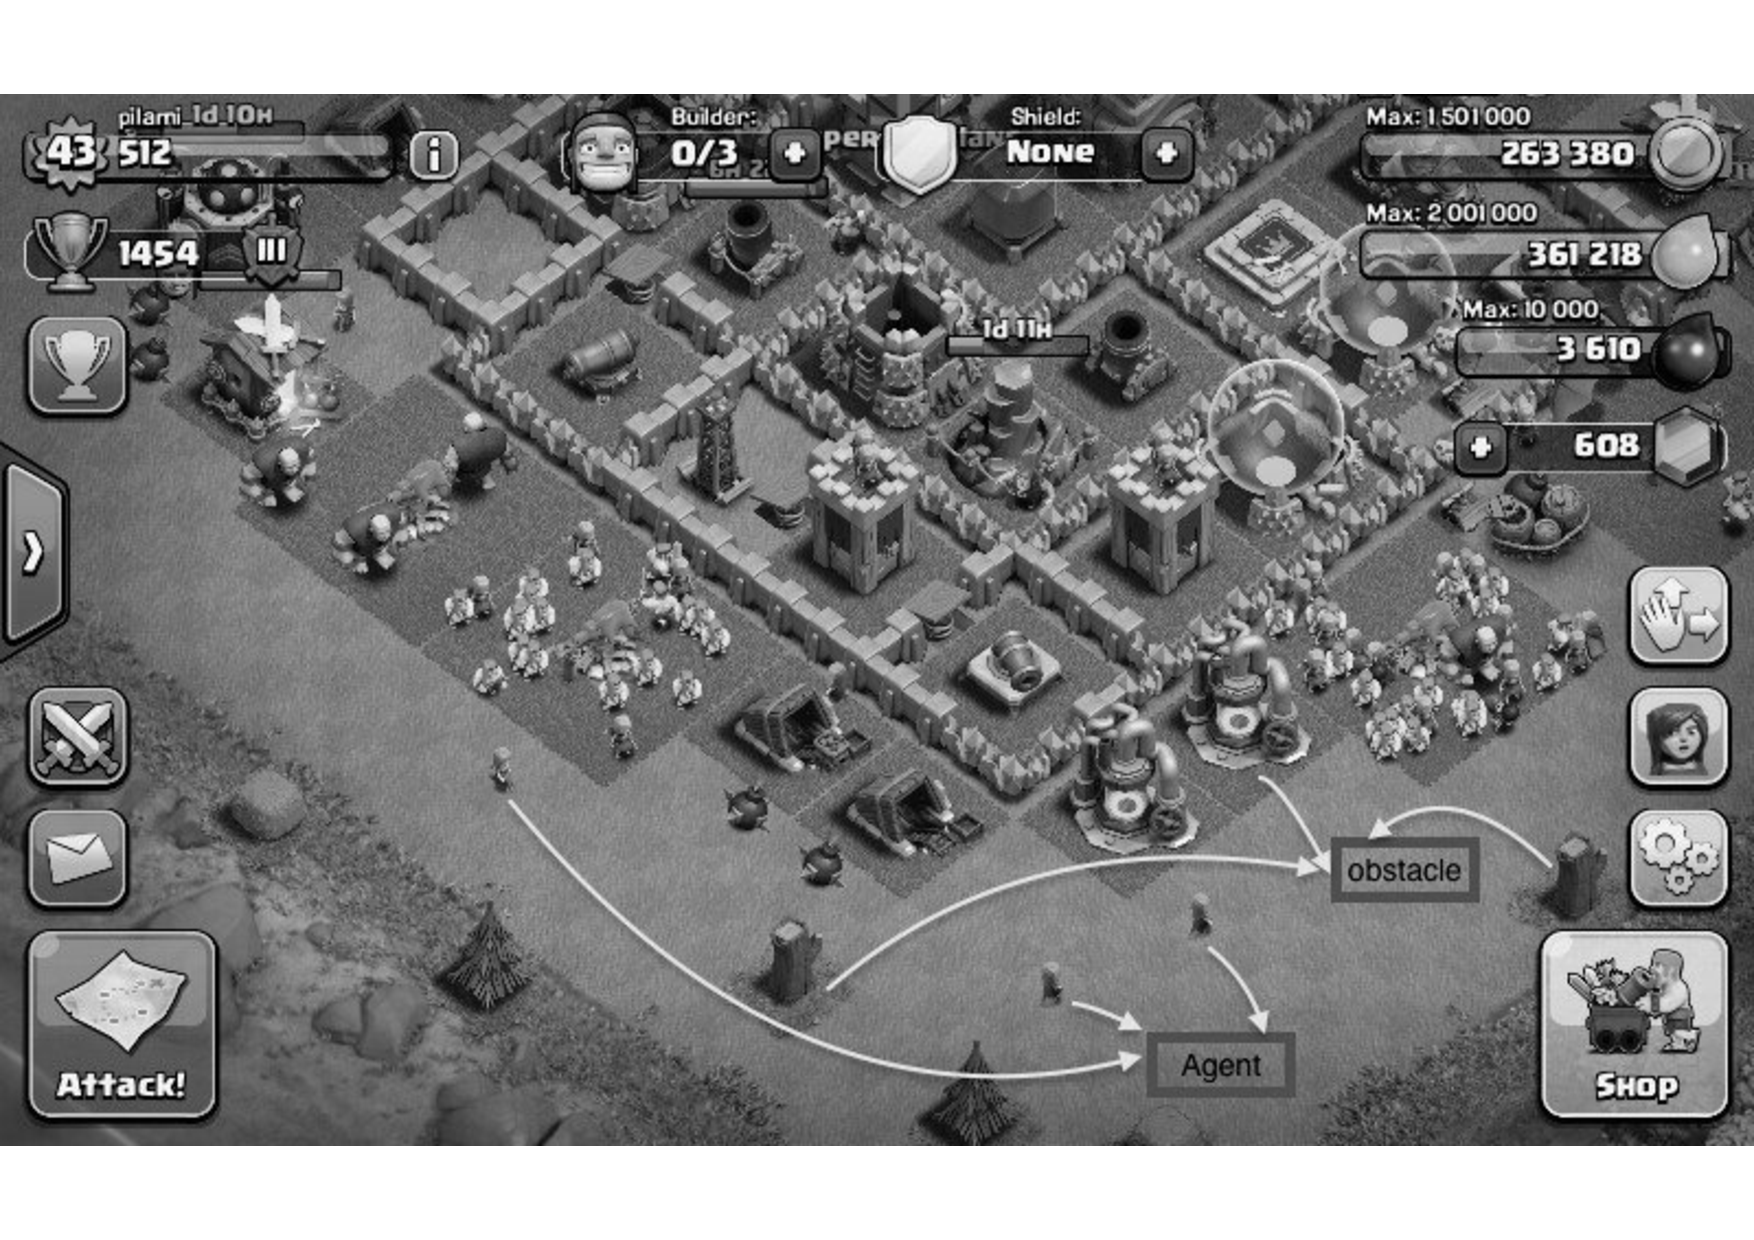
\includegraphics {coc}}
     \resizebox{45mm}{50mm} {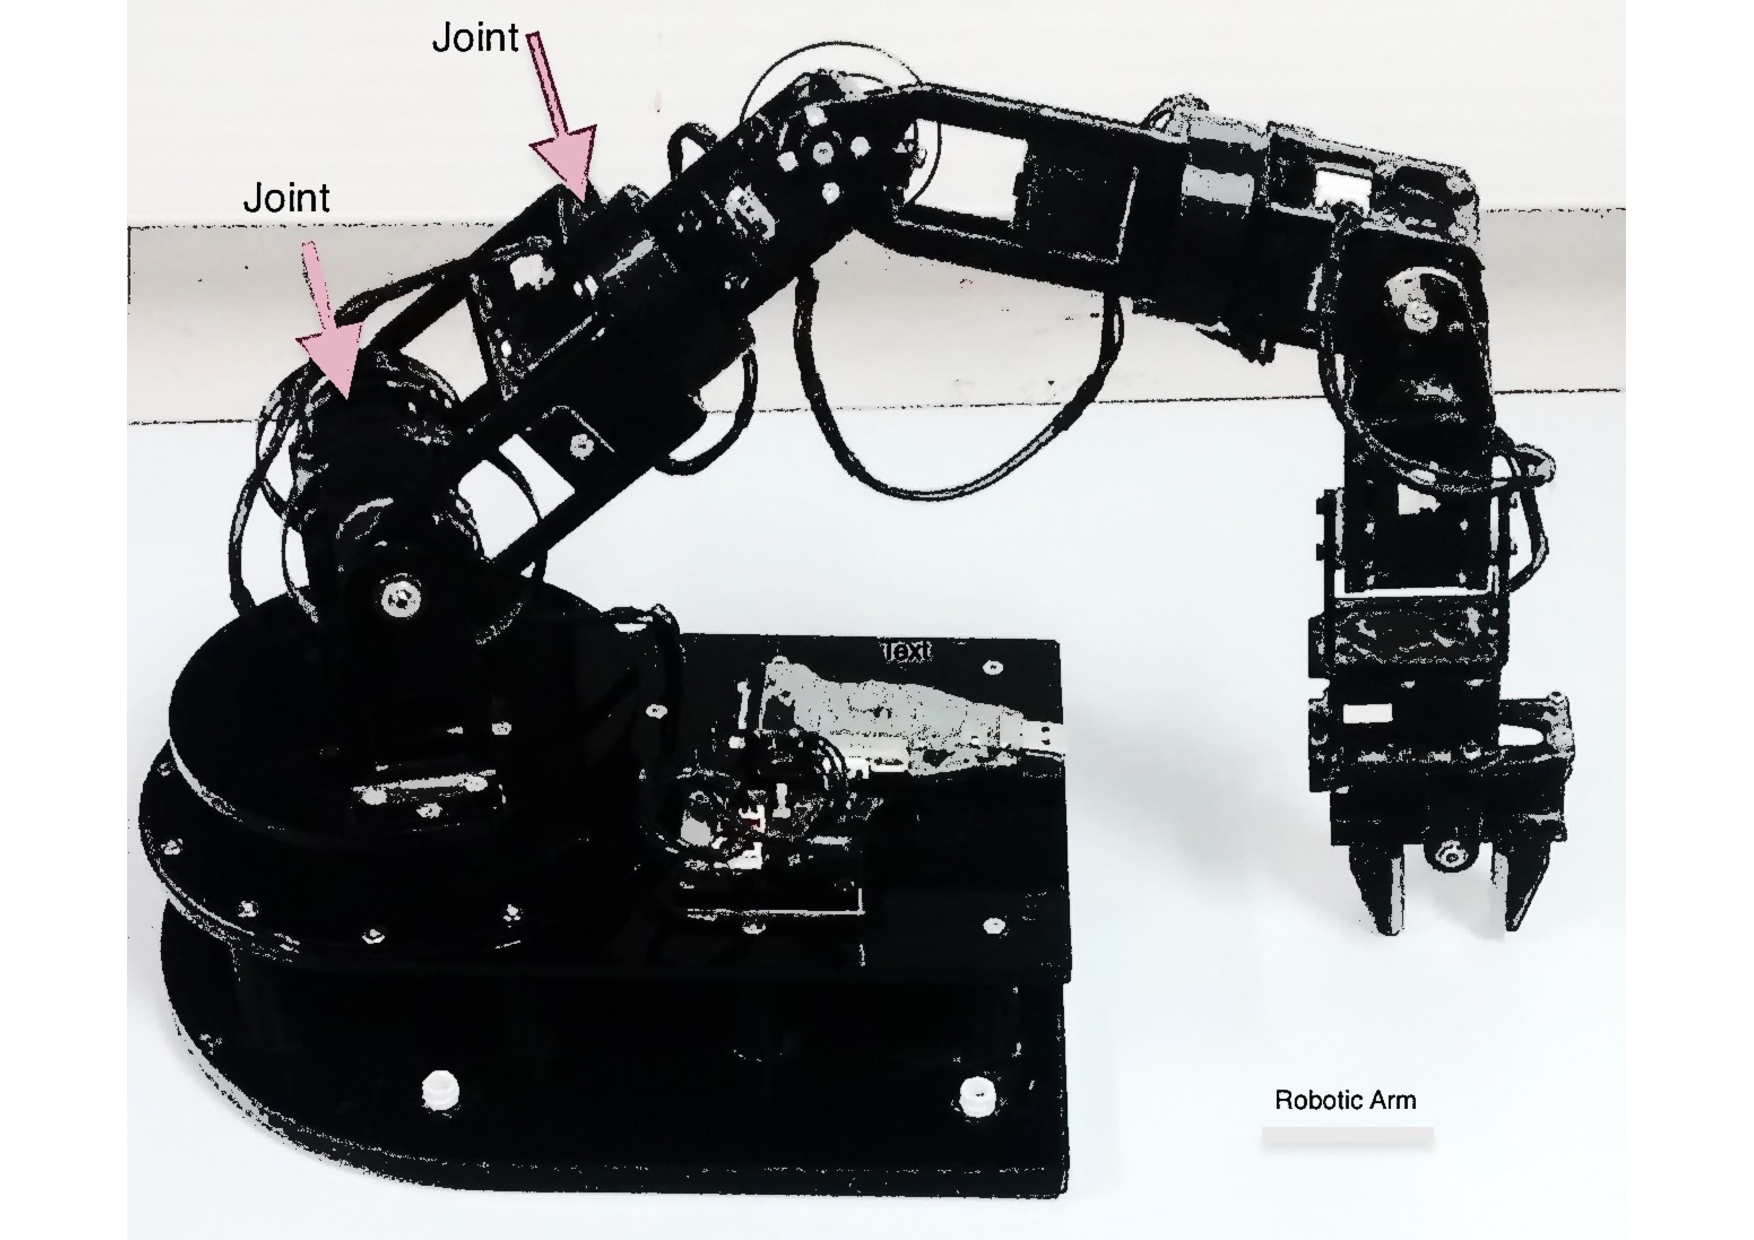
\includegraphics {arm}}
     \caption {Left: screenshot of a game, courtesy: supercell games; Right: 6-D0F Arm}
   \label{fig:coc}
   \end{center}
 \end{figure}
 
	\end{itemize}
}

\frame{\frametitle{Cont. } 
	 Different types
	\begin{itemize}
	\item Known environment 
	\item Unknown environment
	\item Static/Dynamic obstacles
	\item Changing environment 
	\end{itemize}
	Robot entering a room: Continuous state/action spaces, unknown non-stationary environments.
}

\frame{\frametitle{Configuration space} 
\begin{itemize}
\item Description of the geometry of the moving agent or robot.
\item Description of the geometry of the workspace.
\item Description of robot's degrees of freedom.
\item A start and goal configuration( can be set of configurations also)  for the robot.
\end{itemize}
 A solution is now a path connecting points in configuration space. 
\begin{itemize}
\item Kino-dynamic constraints
\item Non-holonomic robot
\end{itemize} 

}

\frame{\frametitle{Approaches. } 
	\begin{itemize}
	\item Search based - Dijkstra, A*, D* ,etc.
	\begin{itemize}
		\item Discretize the space into grid of fixed resolution and work on it.
	\end{itemize}
	\item Potential field based methods
	\begin{itemize}
		\item Potential field across the space and gradient descent.
		\item Local minima. Artificial Randomized Potential Field method. 
		\item Complex environments, large number of obstacles  , keep track of all obstacles
	\end{itemize}
	\item Sampling based methods - PRM, RRT
	\begin{itemize}
	\item Probabilistic Road Maps - multi query not suited for dynamic environment
	\item Rapidly exploring random trees - single shot, space filling, probabilistically complete.
	\end{itemize}
	\end{itemize}
}
\frame{\frametitle{RRT} 
\begin{columns}
        \begin{column}{.5\textwidth}
           \begin{itemize}
				\item Sample a point $x_{random}$
				\item Extend the tree towards the point.
				\begin{itemize}
					\item Find out the "nearest" node to $x_{random}$
					\item Move towards $x_{random}$ by $\epsilon$-distance
				\end{itemize}
			\end{itemize}
        \end{column}        
        \begin{column}{.5\textwidth}\raggedleft
            \begin{figure}[htpb]
			   \begin{center}
		    	 \resizebox{60mm}{50mm} {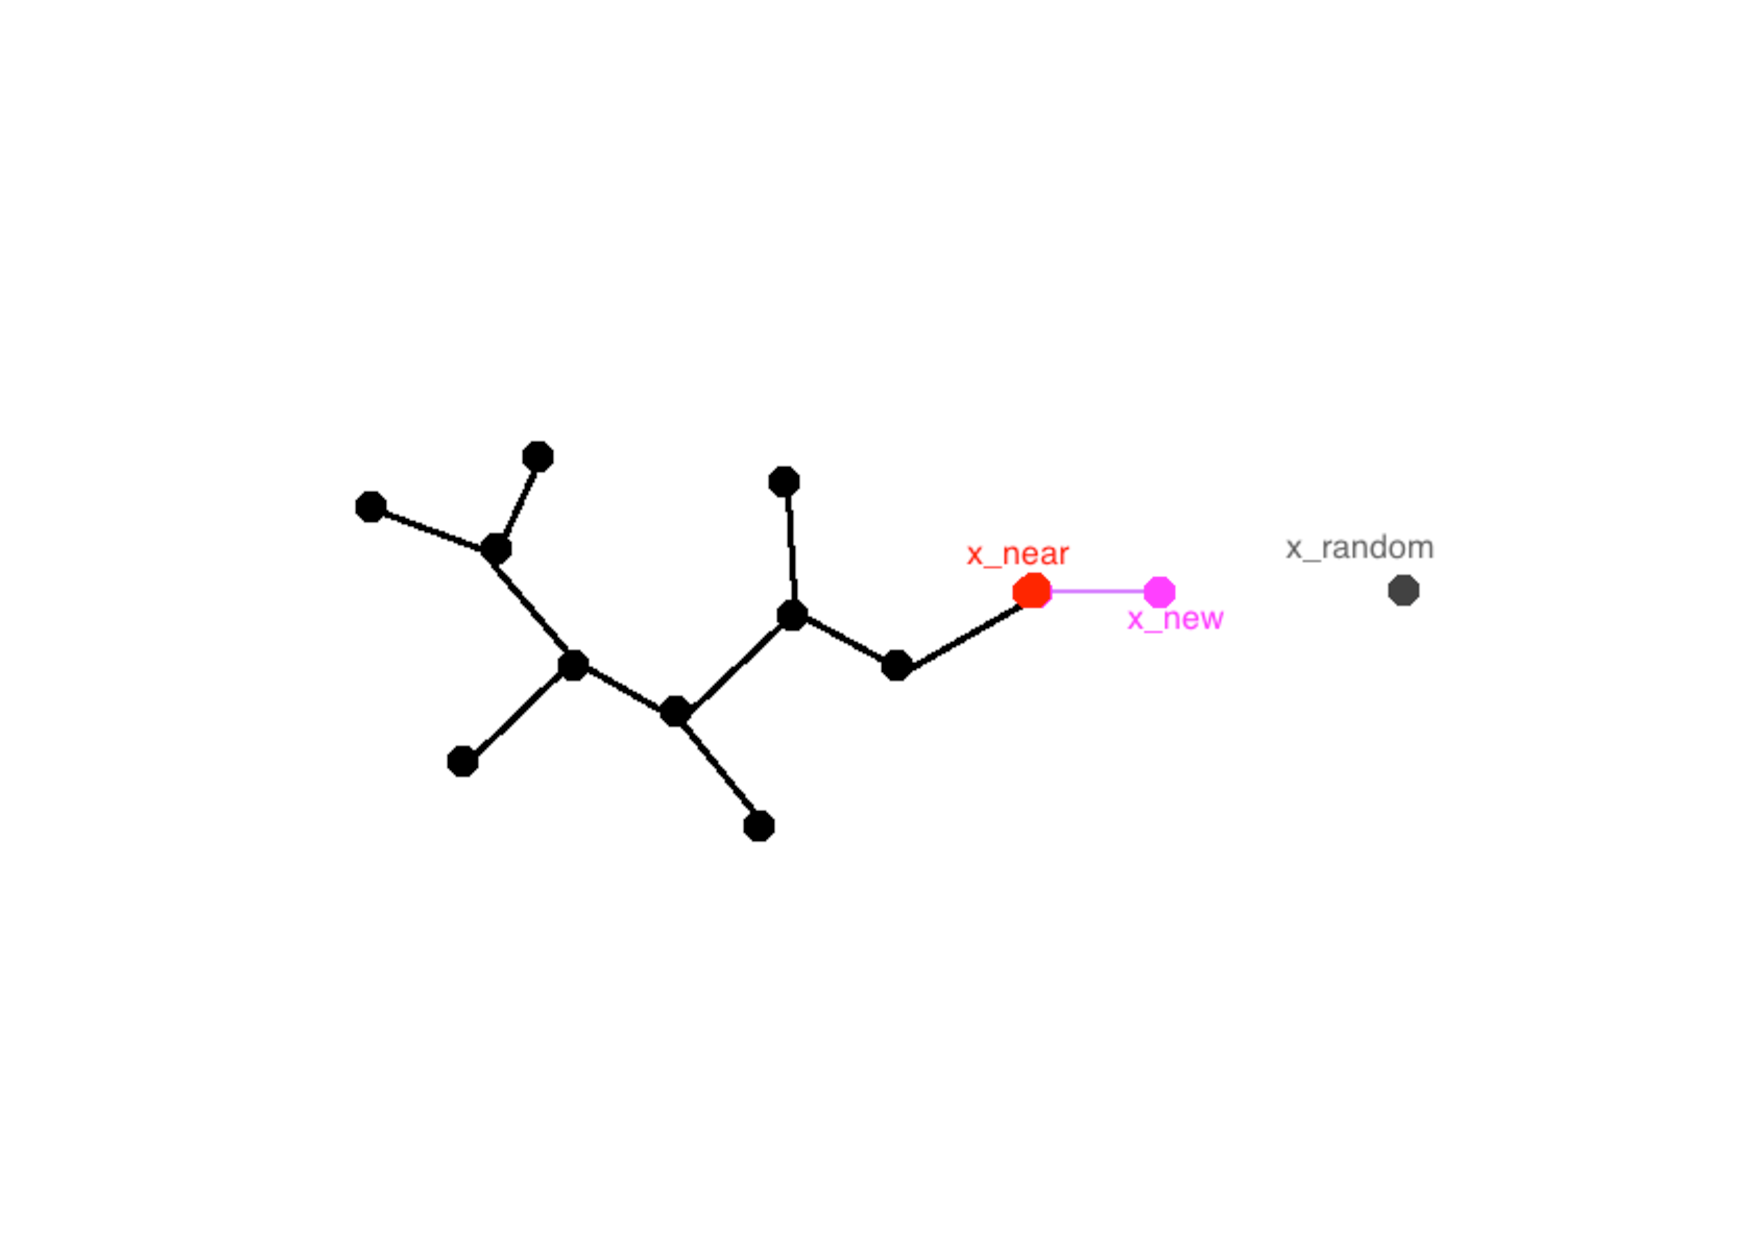
\includegraphics {rrt.pdf}}
			     \caption {RRT extend}
				   \label{fig:rrtextend}
		   		\end{center}
		 \end{figure}
        \end{column}
    \end{columns}
}

\frame{\frametitle{RRT Cont.} 
\begin{columns}
        \begin{column}{.5\textwidth}
           \begin{itemize}
				\item "Rapidly" exploring into voronoi regions.
				\item If large area is unexplored probability of RRT extending into that region is higher than other areas.
			\end{itemize}
        \end{column}        
        \begin{column}{.5\textwidth}\raggedleft
            \begin{figure}[htpb]
   				\begin{center}					  
					 \resizebox{80mm}{50mm} {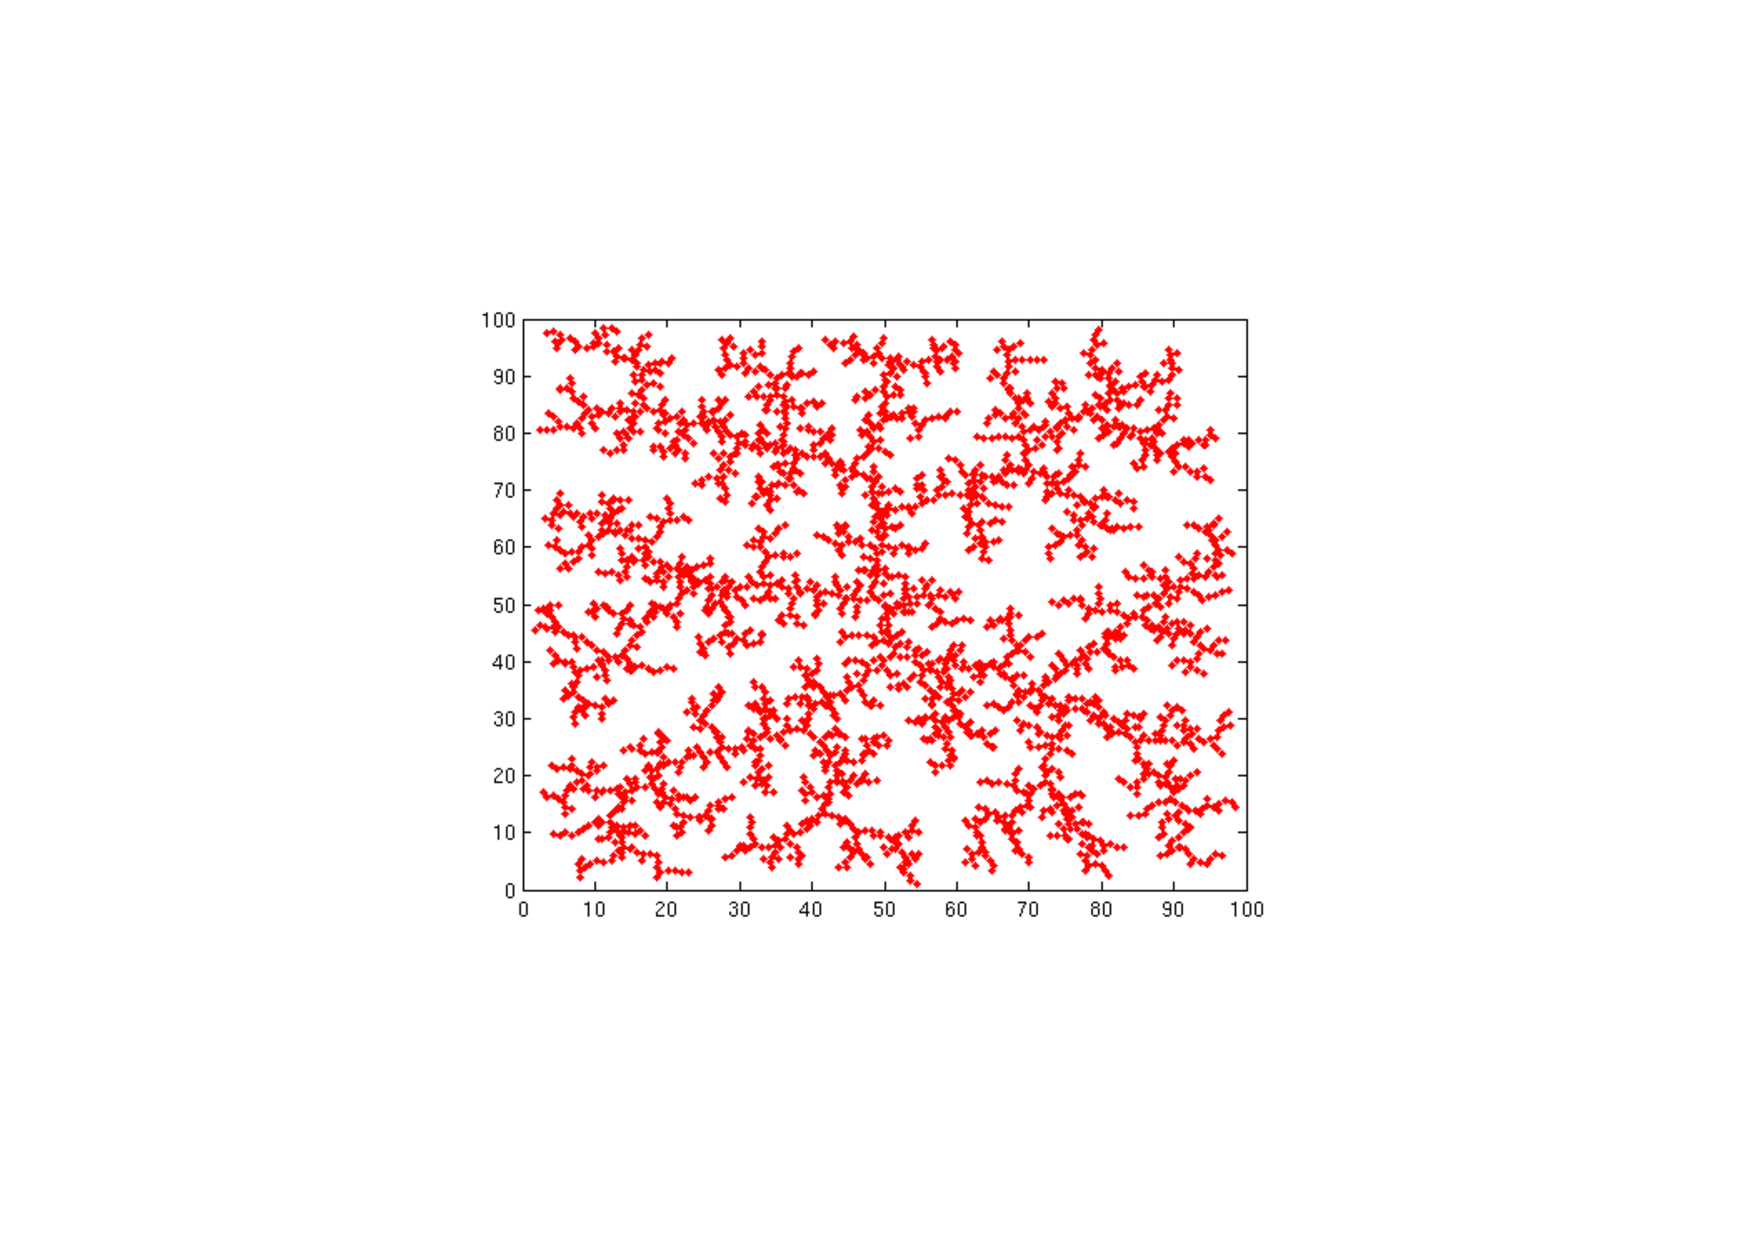
\includegraphics {rrt-basic.pdf}}
				     \caption { A RRT grown from start point [50;50]}
   				\label{fig:rrt-basic}
			  \end{center}
			 \end{figure}
        \end{column}
    \end{columns}
}


\frame{\frametitle{Problems? Motivation!} 
	\begin{itemize}
	\item Takes long time to reach goal.
	\begin{itemize}
		\item goal biasing, RRT-Connect
	\end{itemize}
	\item Sub-optimal solutions
	\begin{itemize}
		\item Heuristic Cost function , RRT*, LQR RRT* , RRT++
		\item But difficult to determine in non-holonomic, high dimensional setups.
	\end{itemize}
	\item Non-stationary environment
	\begin{itemize}
		\item Replanning - E-RRT, D-RRT, MP-RRT.
		\item Potential fields + RRTs. But again issues with potential fields. 
	\end{itemize}
	\end{itemize}
}

\section{DYNA-RRTPI}
\subsection{Preliminaries}
\frame{\frametitle{Reinforcement Learning} 
	\begin{itemize}
	\item We want to learn the distance metric used in RRT procedure using experience.
	\end{itemize}
		 \begin{figure}[htpb]
   				\begin{center}					  
					 \resizebox{50mm}{50mm} {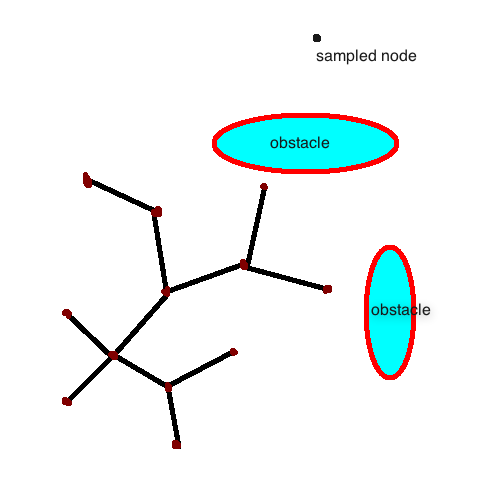
\includegraphics {rrtobstacles}}
					 \resizebox{50mm}{50mm} {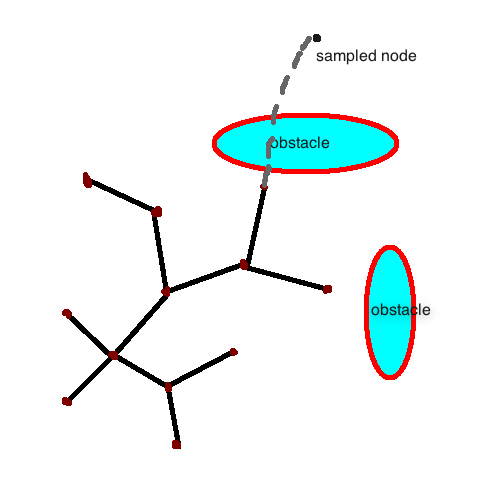
\includegraphics {rrtobstaclesrl}}
				     \caption {RRT: Choose the next point from the tree!}
   				\label{fig:rrt-basic}
			  \end{center}
			 \end{figure}
	}
	\frame{\frametitle{RL} 
	\begin{itemize}
	\item Markov Decision Process (MDP) from RL allows us to learn values of states which are sampled as a chain.
	\item MDP $M$ is a tuple $<S,A,T,R,\gamma>$ where  $S \in R^{n}$ is the $n$-dimensional state space, $A$ is the action space.
	\item Transition function $T(s,a) = s'$. Also $\sum_{\forall s' \in S } T(s,a,s') = 1$ 
	\item $R(s,a,s')$ is the expectation of the real valued rewards for action  $a \in$ $A$
	\item For a trajectory $s_o, a_o,r_1, s_1,a_1.r_2,s_2, a_2,r_3,s_3... $\\
	 Return = $\displaystyle \sum_{t=0}^{\infty} \gamma^t r_t$, where $r_t $ is the reward at the time step t 
	\item A policy $\pi$ is a mapping from state space $S$ to action space $A$ $\pi:S$x$A \rightarrow [0,1]$ and 
	  $\pi(s) = a$	
	\end{itemize}
}

\frame{\frametitle{Solving MDP} 
	\begin{itemize}
	\item State value function $J^{\pi}(s)$ is the expected return from any state $s$
	\item Optimal Policy: $ \pi ,\forall s\in S, $ $J^{\pi}(s) < J^{\pi^*}(s)$,
	\item Bellman equation $$J^{\pi}(s) = \displaystyle \sum_{a}\pi(s,a) \sum_{s'}T(s,a,s')[ R(s,a,s')+ \gamma J^{\pi}(s') ] $$
	\item T and R are not available readily.
	\end{itemize}
}
	\frame{\frametitle{Solving MDP} 
	\begin{itemize}
	
	\item  Sampling trajectories $\{s_o,a_o,r_1,s_1,a_1,r_2,s_2,... s_M\}_{i=1}^N$
	\item TD(0) update rule 
	$$J^{\pi}(s_t) = (1 - \alpha) J^{\pi}(s_t) + \alpha (r_t + \gamma J^{\pi}(s_{t+1})) $$ 
	$\alpha $ step size and $\gamma$ discount factor 
	\end{itemize}
	 \begin{figure}[htpb]
   				\begin{center}					  
					 \resizebox{40mm}{40mm} {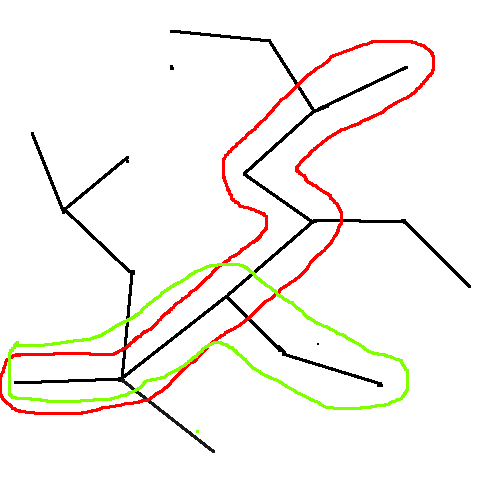
\includegraphics {rrtmdp}}
				     \caption {RRT: TD(0) on RRTs}
   				\label{fig:rrtmdp}
			  \end{center}
			 \end{figure}	
}

\frame{\frametitle{DYNA} 

	\begin{itemize}
		\item In dynamic domains, agent should quickly repond to changes
		\item Integrate planning and execution
		\item Action taken is used to update J function as well as maintain a model and do simulated planning.
	\end{itemize}
	 \begin{figure}[htpb]
   				\begin{center}					  
					 \resizebox{80mm}{40mm} {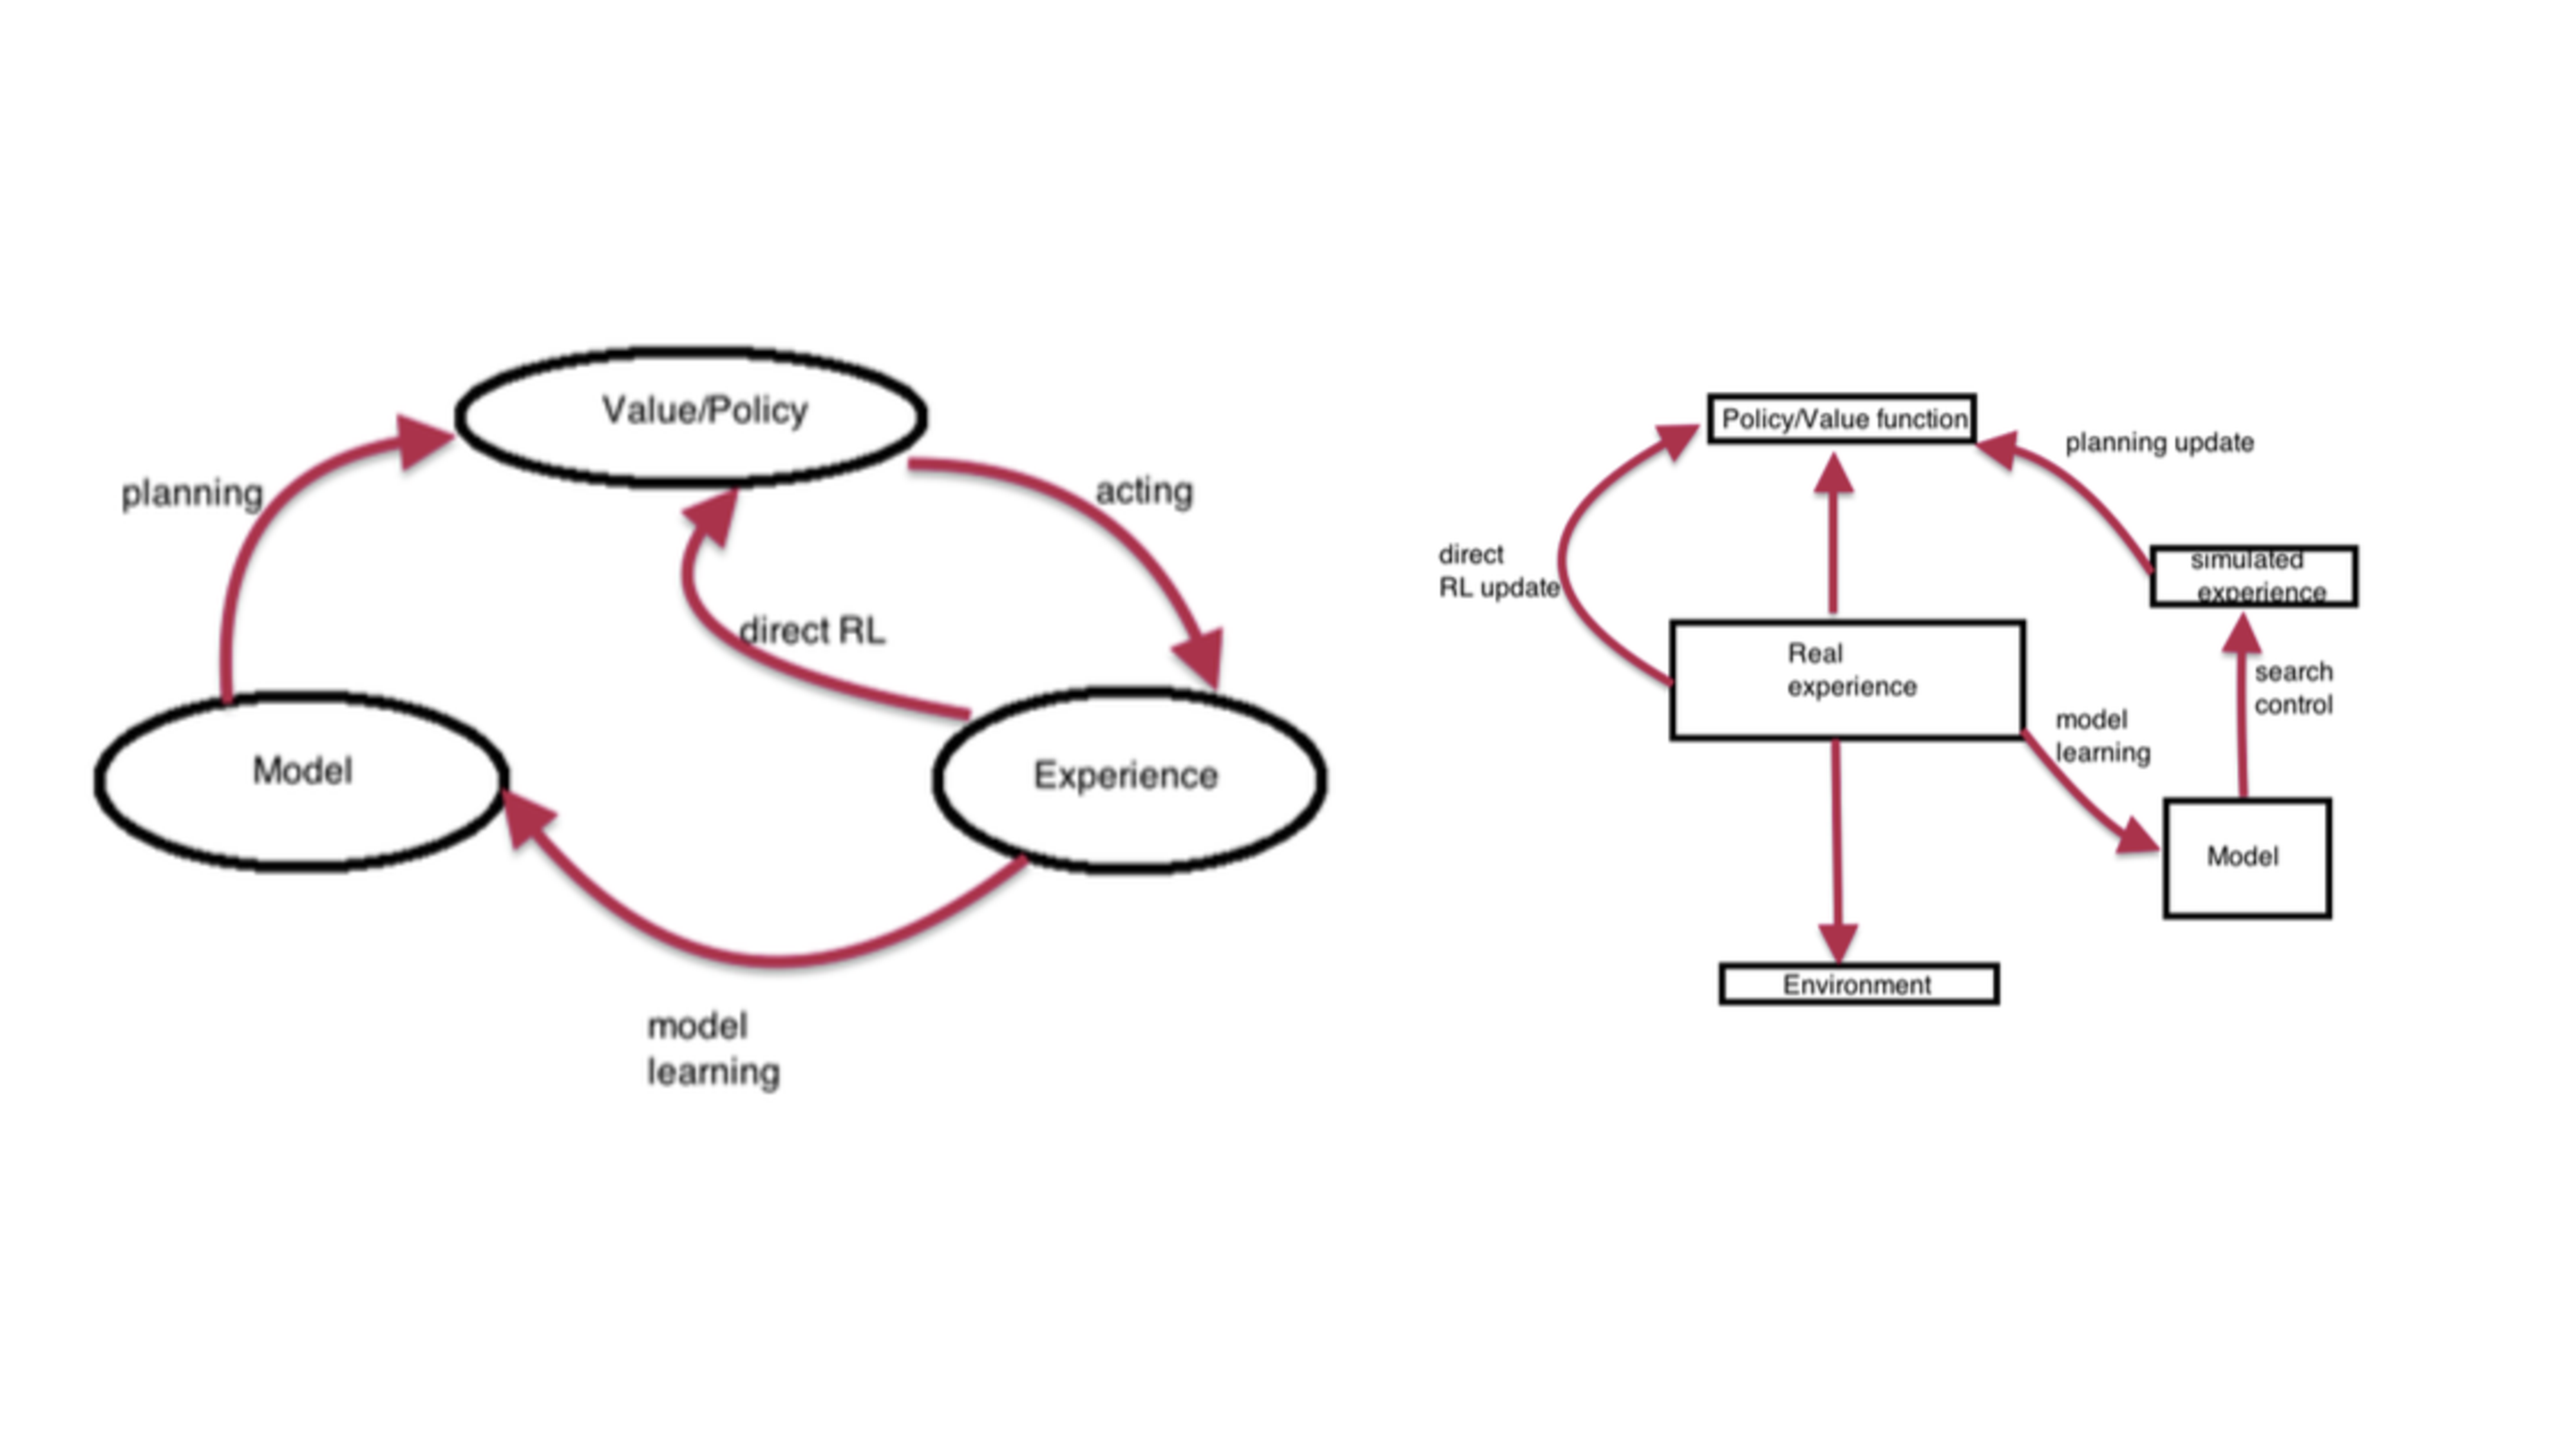
\includegraphics {dyna}}
				     \caption { Relationship between Value function , Experience and Models and DYNA framework}
   				\label{fig:dyna}
			  \end{center}
			 \end{figure}

}
\subsection{Algorithm}

\frame{\frametitle{DYNA-RRTPI} 
We present algorithms for Episodic, Online, Dynamic Replanning settings.
%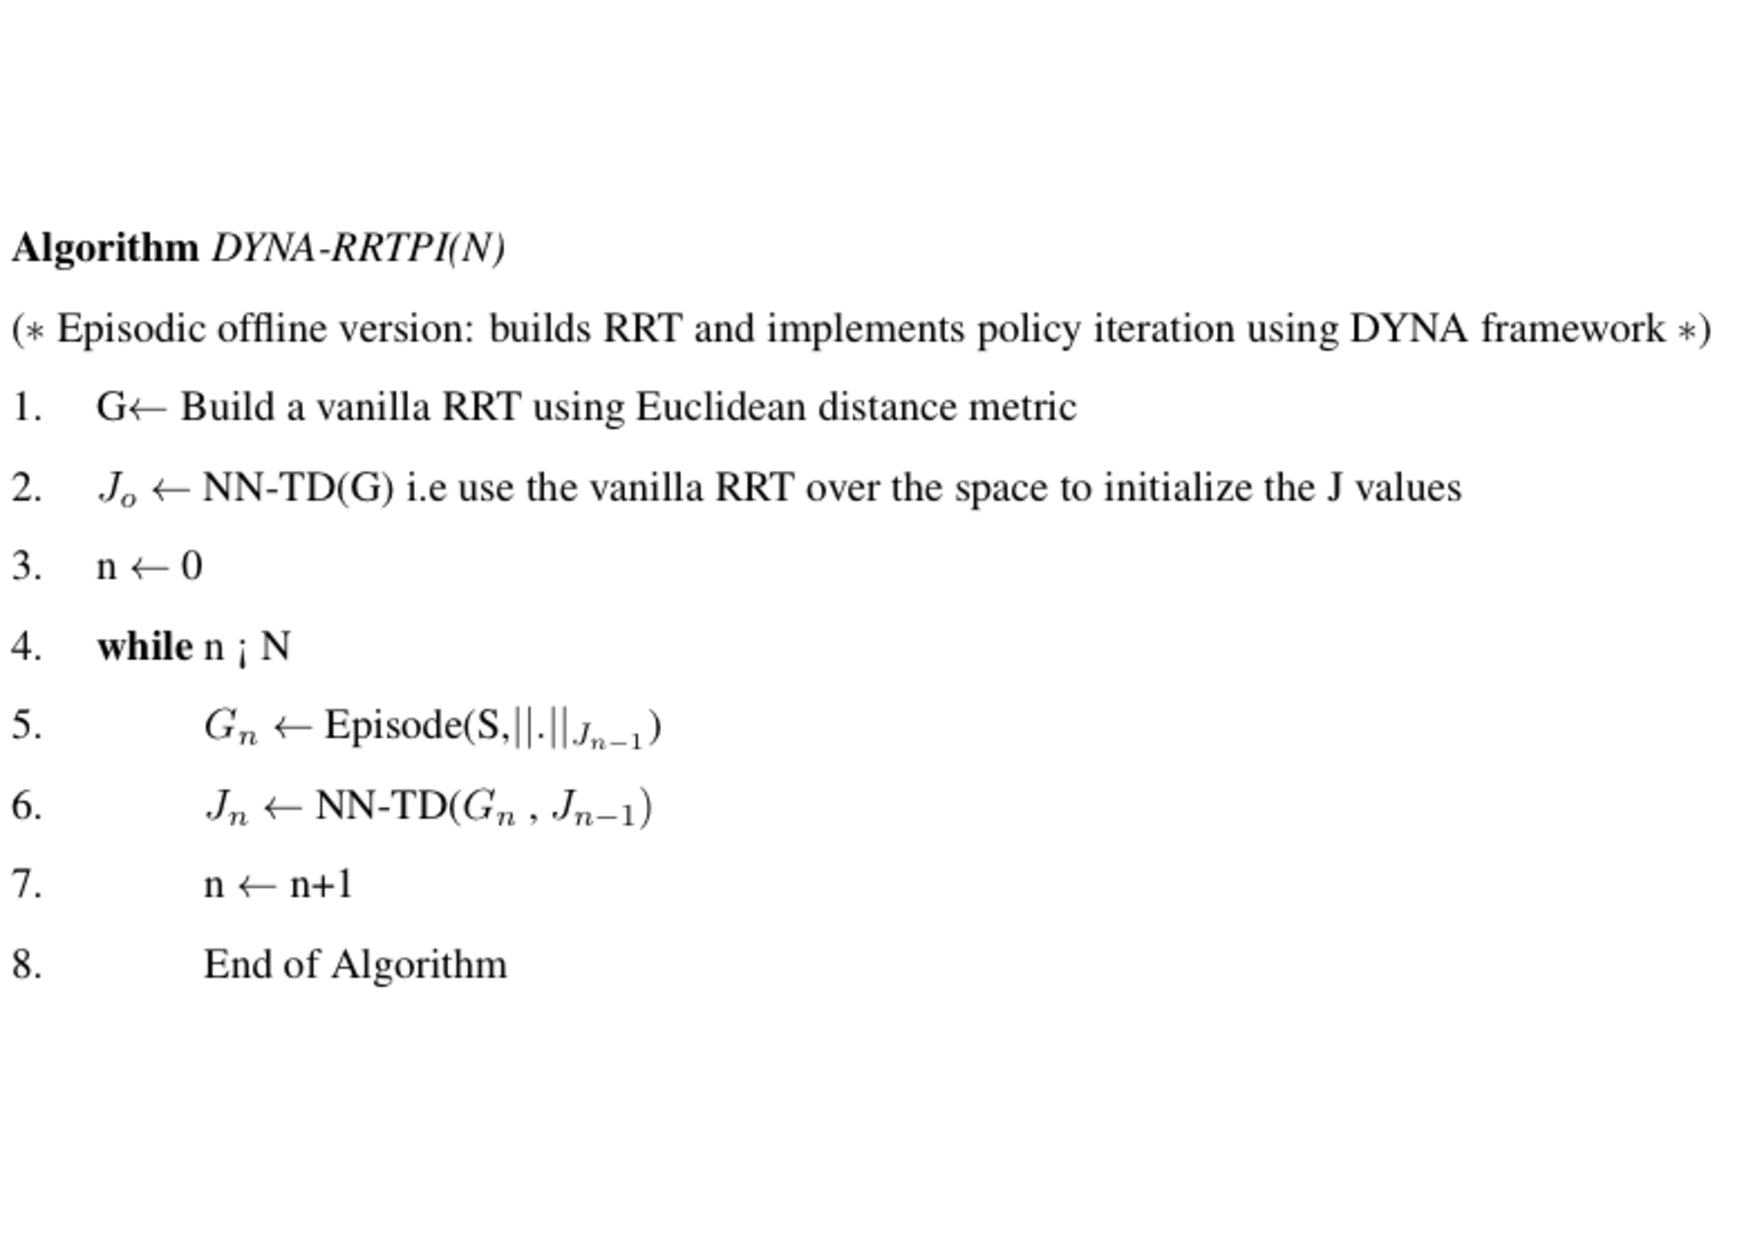
\includegraphics[scale=0.3]{episodicrrtpi}
\begin{algorithm}{DYNA-RRTPI(N)}{
\label{algo:DYNA-RRTPI}
\qcomment{Episodic offline version}}
G$\leftarrow$ Build a vanilla RRT using Euclidean distance metric\\
$J_o \leftarrow$ NN-TD(G) i.e use the vanilla RRT over the space to initialize the J values\\ 
n $\leftarrow$ 0\\
\qwhile n $<$ N \\
$G_n \leftarrow$ Episode(S,$ || . ||_{J_{n-1}} $)\\
$J_n \leftarrow$ NN-TD($G_n$ , $J_{n-1})$ \\
n $\leftarrow$ n+1\qend\\
End of Algorithm
\end{algorithm}
}

\frame{\frametitle{Policy Improvement } 
\begin{algorithm}{Episode(S, $|| . ||_J$)}{
\label{algo:Dyna-Episode}
\qcomment{Build a RRT using value functions in dyna framework }}
 V(G) $\leftarrow$ {$x_{start}$};  E(G) $\leftarrow${$\phi$ } \\
\qwhile goal is not reached \\
$x_{rand}$ $\leftarrow$ Sample(S);\\
$x_{near}$ $\leftarrow$ Modified-Nearest($x_{rand}$, V(G) , $|| . ||_J $ );\\
$(x_{new}, a, r) \leftarrow$ Extend($x_{near}$, $x_{rand}$, S);\\
\qif Not-Colliding($x_{new}$, $x_{near}$,S)\\
\qthen Connect $x_{new}$ to $x_{near}$\\
V(G) $\leftarrow$ V(G) U {$ x_{new}$ }\\
E(G) $\leftarrow$ E(G) U ($x_{new}, a, r$)\\
$J(x_{near}) \leftarrow (1 - \alpha) J (x_{near} + \alpha (r + \gamma J(x_{new})))$ \qfi\\
J $\leftarrow$ RRT-Planning(G, J, number of iteration)\qend\\
return G\\
End of Algorithm
\end{algorithm}
}

\frame{\frametitle{Policy Evaluation} 
We estimate the value function from the trajectories using TD-learning
\begin{algorithm}{NN-TD(G, J)}{
\label{algo:NN-TD}
\qcomment{Estimates the value function J from the trajectories}}
Let $Y_n$ be the set of trajectories starting at $x_start$ till leaf nodes in G.\\
\qfor each trajectory $(s_o, a_o, r_1, s_1, a_1, r_2, s_2, ...)$ in $Y_n$\\
\qfor each pair $(s_i,a_i,r_{i+1}, s_{i+1})$\\
$J(s_i) = (1 - \alpha) J(s_i) + \alpha(r_i + \gamma J(s_{i+1})$\qrof\qrof\\
return J\qend\\
End of Algorithm
\end{algorithm}
}


\frame{\frametitle{Nearest Point}
\begin{itemize}
\item The basic nearest procedure in does not work well.
\item We modified the procedure to work with any intialization. We use euclidean distance to sort the points whose J values are close. 
\end{itemize}
\begin{algorithm}{Modified-Nearest($x_{rand}$, V(G) , $|| . ||_J$ )}{
\label{algo: Modified-Nearest}
\qcomment{Finds a point nearest to given point in the graph }}
 $X_{near} \leftarrow$ subset of vertices in V(G) such that  $x_{near} = \displaystyle arg\max_{x \in V(G)} (|| x - x_{rand}|| ) $\\
 return $x_{near} \in X_{near}$ that is closest to the goal when compared using euclidean distance\\
End of Algorithm
\end{algorithm}
$||x - y||_J$ = $J(x) - J(y)$ where x, y $\in$ S.
}
\frame{\frametitle{Extend }
\begin{algorithm}{Extend($x_{near}$, $x_{rand}$, S)}{
\label{algo:Extend}
\qcomment{Finds a point close to $x_{rand}$ that is in $\epsilon-$neighbourhood of $x_{near}$} respecting the kinodynamic constraints}
 $x_{new} \leftarrow$  $\displaystyle arg\max_{a \in A} ||x - x_{rand} ||_J$ and $|| x_{new} - x_{near} ||$ is within kinematic bounds and action $a_{max}$ which generated $x_{new}$ is within the acceleration bounds\\
 $(r,x_{new} ) \leftarrow$ MDP($x_{near}$,a)\\ 
 return ($x_new, a, r$)\\
End of Algorithm
\end{algorithm}
}

\frame{\frametitle{Planning }

\begin{algorithm}{RRT-Planning(G, $|| . ||_J$, number of iterations)}{
\label{algo:Simulate RRT sampling trajectories from given rrt and update value function}
\qcomment{samples trajectories using RRTs}}
n $\leftarrow$ 0\\
\qwhile n $<$ number of iterations\\
Randomly sample a point $x_{begin}$ from V(G)\\
Find a trajectory $Y$ with $x_{begin}$ as the root\\
\qfor each pair $(s_i,a_i,r_{i+1}, s_{i+1}) \in Y$\\
$J(s_i) = (1 - \alpha) J(s_i) + \alpha(r_i + \gamma J(s_{i+1})$\qrof\qend\\
return J\\
End of Algorithm
\end{algorithm}
}


\frame{\frametitle {Replanning in DYNA-RRTPI}

\begin{algorithm}{Replan-DYNA-RRTPI( )}{
\label{algo:Replan-DYNA-RRTPI}
}
%G$\leftarrow$ Build a vanilla RRT using Euclidean distance metric\\
F $\leftarrow$ initialize to empty set of forest of disconnected trees.
%$J_o \leftarrow$ NN-TD(G) i.e use the vanilla RRT over the space to initialize the J values\\ 
\qwhile Graph G doesnt contain goal \\
\qif Graph is not empty \\
\qthen Prune(G,F)\\
\qelse Intialize V(G) $\leftarrow$ $\{x_{start} \}$\qfi\\
$x_{rand}$ $\leftarrow$ Modified-Sample(S,F);\\
$x_{near}$ $\leftarrow$ Modified-Nearest($x_{rand}$, V(G) , $|| . ||_J $ );\\
$(x_{new}, a, r) \leftarrow$ Extend($x_{near}$, $x_{rand}$, S);\\
\qif Not-Colliding($x_{new}$, $x_{near}$,S)\\
\qthen Connect $x_{new}$ to $x_{near}$\\
V(G) $\leftarrow$ V(G) U {$ x_{new}$ }\\
E(G) $\leftarrow$ E(G) U ($x_{new}, a, r$)\\
$J(x_{near}) \leftarrow (1 - \alpha) J (x_{near} + \alpha (r + \gamma J(x_{new})))$ \qfi\\
J $\leftarrow$ RRT-Planning(G, J, number of iteration)\qend
\end{algorithm}



}

\frame{ \frametitle{Prune}
\begin{algorithm}{Prune(Graph G, Forest F)}{
\label{algo:Prune}
\qcomment{Perfoms collision checks on all nodes and removes nodes }}
\qfor each node q $\in$ V(G) and F\\
\qif Not-valid (q)\\
\qthen remove q from G and F\\
split the tree at q and add subtrees to F\qfi\qrof\\
\qif G is empty \\
\qthen Initialize G and add $x_{start}$ to V(G)\qfi\\
End of Algorithm
\end{algorithm}
}

\frame{\frametitle{Sampling}
\begin{algorithm}{Modified-Sample(S,F)}{
\label{algo: Modified-Sample}
\qcomment{Returns a point to which the RRT would try to expand to}}
prob $\leftarrow$ Random(0,1)\\
\qif prob $<$ $p_{goal}$\\
\qthen $x_{result}$ $\leftarrow$ $x_{goal}$\\
\qelse \qif prob $< p_{goal} + p_{forest}$\\
\qthen $x_{result} \leftarrow$ root of a randomly sampled tree from $F$ , the forest of disconnected trees.\\
\qelse $x_{result}$ $\leftarrow$ Randomly sample a point from the state space \qfi\qfi\\
return $x_{result}$\\
End of Algorithm
\end{algorithm}
}



\subsection{Experiments}
\frame{\frametitle{Continuous Domain} 
	\begin{itemize}
		\item We test our algorithm against RRTPI in continuous puddle world domain.
		\begin{itemize}
			\item continuous space (0,0) to (50,50). Start at (5,5) and goal is to reach above (45,45). one puddle of radius 5 at (30,10)
		\end{itemize}
		\begin{figure}[htpb]
   \begin{center}
     \resizebox{35mm}{30mm} {\includegraphics *{dyna3}}
      \resizebox{35mm}{30mm} {\includegraphics *{rrtpi40}}
     \caption { The value function distribution for the puddle world task.  The green line is the path learnt in RRT grown in that episode. The left graph is for 3 episodes of DYNA-RRTPI and right graph for RRTPI.}. 
     \label{puddleworldvalue}
     \end{center}
     \end{figure}
	\end{itemize}		

}
\frame{\frametitle{Cont.}

\begin{figure}[htpb]
   \begin{center}
     \resizebox{100mm}{50mm} {\includegraphics *{continuouspuddleworld}}
     \caption {DYNARRTPI vs RRTPI in 2-D continuous puddle world from (0,0) to (50,50) with puddle of radius 5 at (30,10) }. 
     \label{continuouspuddleworld}
     \end{center}
     \end{figure}

}
\frame{\frametitle{Dynamic Environment}
\begin{itemize}
	\item We increased the puddle radius after the algorithms have estimated the value functions.
\end{itemize}
\begin{figure}[htpb]
   \begin{center}
     \resizebox{35mm}{40mm} {\includegraphics *{rrtpibeforechange}}
      \resizebox{35mm}{40mm} {\includegraphics *{rrtpiafterchange}}
       \resizebox{35mm}{40mm} {\includegraphics *{rrtpiafter10episodes}}
     \caption {from left to right, RRTPI before puddle expansion, RRTPI in the episode after puddle expansion and RRTPI after 10 episodes }. 
     \label{dynapuddlemove}
     \end{center}
     \end{figure}
}

\frame{\frametitle{DYNA-RRTPI}

	\begin{figure}[htpb]
   \begin{center}
     \resizebox{50mm}{50mm} {\includegraphics *{dynabeforechange}}
      \resizebox{50mm}{50mm} {\includegraphics *{dynaafterchange}}
     \caption { DYNA-RRTPI in successive episodes when puddle radius is increased. }. 
     \label{dynapuddlemove}
     \end{center}
     \end{figure}
}


\section{Conclusion}
\frame{\frametitle{Conclusion and Future work} 
	\begin{itemize}
	\item We present DYNA-RRTPI which gives near optimal paths combining good qualities of RRTs , RL, efficient replanning techniques.
	\item Responsive algorithm to dynamic changes
	\item Online algorithm - learn when its deployed
	\item Works in continuous space domains also and does not need explicit representation of enivironment and other obstacles
	\item Next, it can be tested on a real world robot navigation or a high dimensional problem like 6-DoF robotic arm.
	\end{itemize}
}
\frame{\frametitle{Appendix}
\begin{itemize}
\item Appendix
\end{itemize}

}

\frame{\frametitle{Online DYNA-RRTPI}
\begin{algorithm}{Online-DYNA-RRTPI( )}
%\label{algo:Online DYNA-RRTPI}
%\qcomment{Online version: builds RRT and implements policy iteration using DYNA framework}}
.$G \leftarrow$ Build a vanilla RRT using Euclidean distance metric\\
$J_o \leftarrow$ NN-TD(G) i.e use the vanilla RRT over the space to initialize the J values\\ 
\qwhile goal is not reached  \\
$x_{rand}$ $\leftarrow$ Sample(S);\\
$x_{near}$ $\leftarrow$ Nearest($x_{rand}$, V(G) , $|| . ||_J $ );\\
$(x_{new}, a, r) \leftarrow$ Extend($x_{near}$, $x_{rand}$, S);\\
\qif Not-Colliding($x_{new}$, $x_{near}$,S)\\
\qthen Connect $x_{new}$ to $x_{near}$\\
V(G) $\leftarrow$ V(G) U {$ x_{new}$ }\\
E(G) $\leftarrow$ E(G) U ($x_{new}, a, r$)\\
$J(x_{near}) \leftarrow (1 - \alpha) J (x_{near} + \alpha (r + \gamma J(x_{new})))$ \qfi\\
J $\leftarrow$ RRT-Planning(G, J, number of iteration)\qend\\
End of Algorithm
\end{algorithm}
}

\frame{\frametitle{Discrete Domain Experiments} 
	\begin{itemize}
	\item Implemented on a discrete grid world domain. 15x15 grid, 100 episodes , maximum iterations 200 per episode and 50 per planning step. Both RRTPI and DYNA-RRTPI converge to the best solution. 
	\item Increased the maximum iteration limit for RRTPI as it does not take time in planning step.
	\end{itemize}
}


\frame{\frametitle{Continued} 

		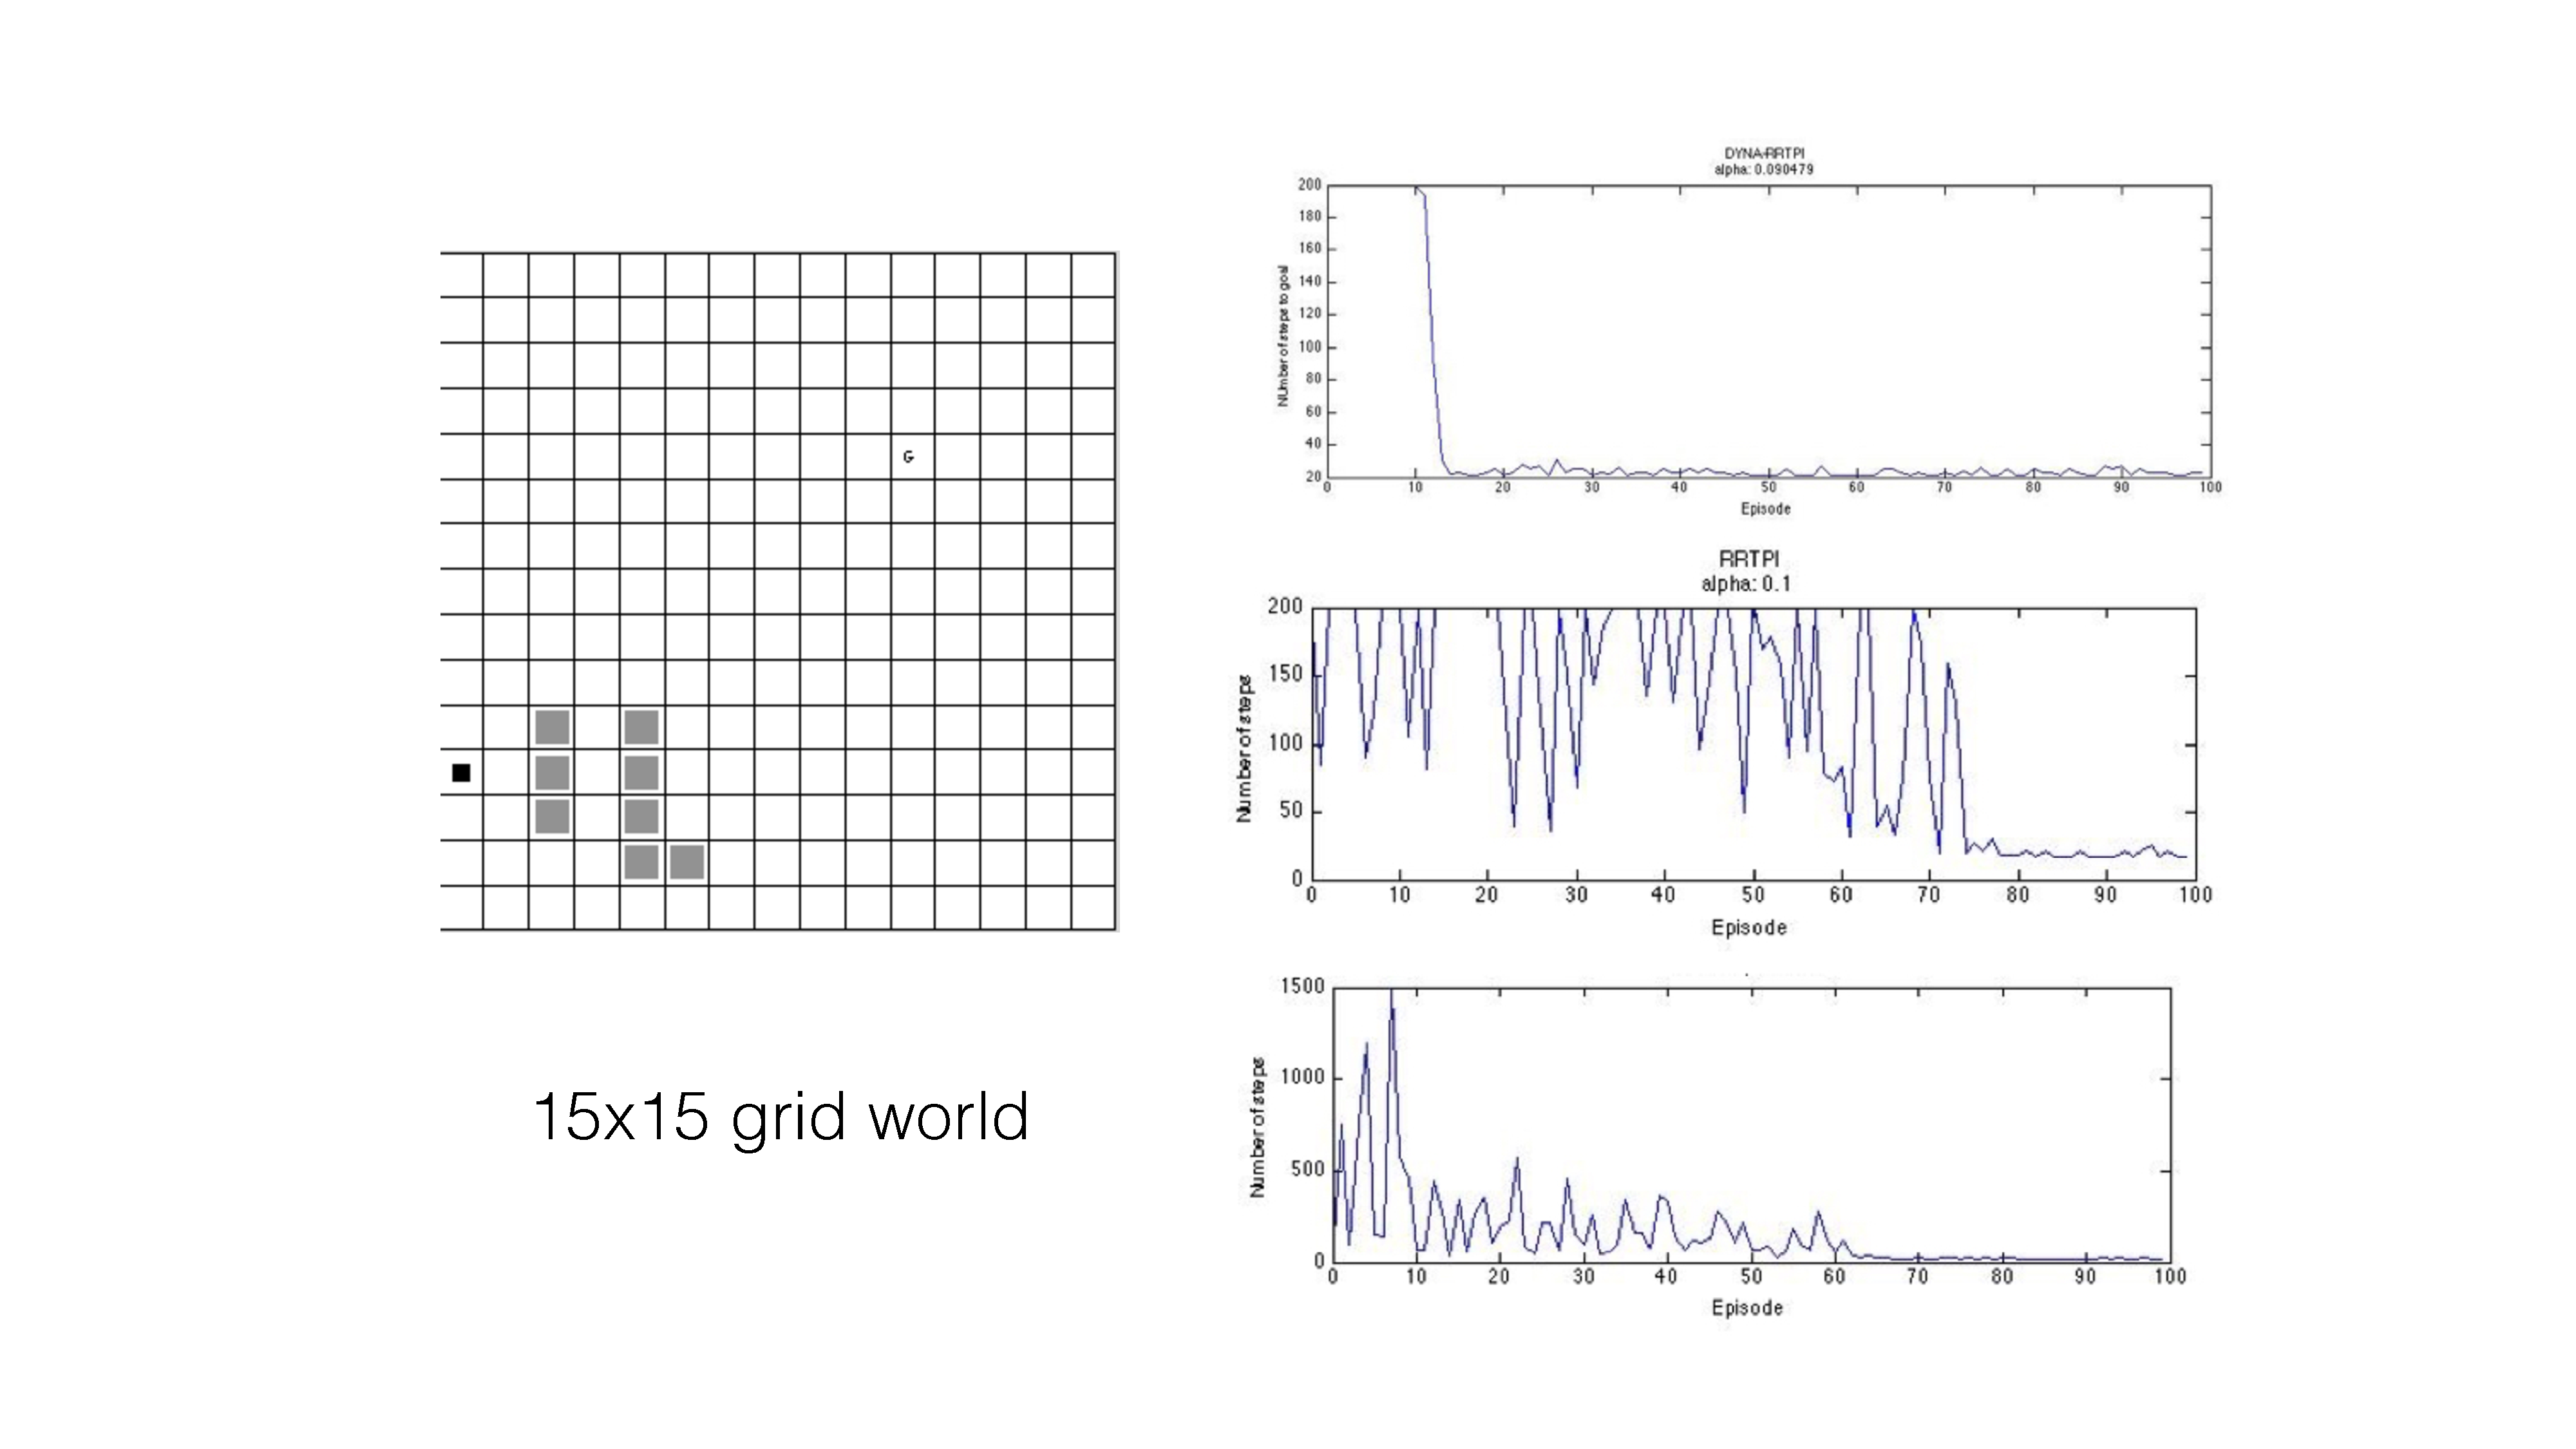
\includegraphics[scale=0.15]{discretefinal}\\
		figure: Number of steps taken to reach goal vs Episode in DYNA-RRTPI and RRTPI

}

\end{document}